\chapter{针对移动相机的快速视频背景减除技术}
 \label{ch4:FMCBS}
 本章对移动相机情况下的视频背景减除技术进行了研究,提出了一种针对移动相机的基于无参数模型的快速视频背景减除算法。该算法主要利用两方面的线索得到视频中准确的前景对象。首先引入最相似变换(as-similar-as-possible warping, ASAPW)方法对相机的运动进行估算和补偿,利用无参数的采样背景模型进行背景建模,利用背景模型这一前景外观线索获得粗略的前景结果。与目前已有的其他方法不同的是,本章所提出的算法不需要计算稠密光流或像素点轨迹等预处理过程,而是通过本章提出的基于超像素的区域增长算法(superpixel-based seeded region growing, SSRG) 将基于稀疏光流的前景线索扩散到整幅图像范围,获得另外一个基于运动线索的粗略前景结果。最后通过基于超像素的马尔可夫随机场(Markov random field, MRF)优化过程对两种线索得到的粗略结果进行优化,最终获得准确的前景。大量实验证明了本章所提出算法的有效性,与目前领先的算法相比本章算法可以得到与之相近的前景准确度;但在计算速度方面,本章所提出的算法要快得多。

 \section{研究背景}
 \label{ch4:sec:background}
视频背景减除技术,或移动目标检测技术,的目的是将视频图像序列中每帧图像当中的移动前景和背景部分分离。该技术已经广泛应用于视频监控、目标跟踪、动作识别等领域。此外,该技术通常作为其他计算机视觉和计算机图形学应用的预处理步骤。例如,在机器人的自主导航中,需要预先将摄像头拍摄的视频中的前景和背景部分分离,提取后续工作中需要用到的前景目标。早期的视频背景减除技术研究当中,一般假定相机在拍摄视频时是静止的。在这种假设下,区分视频中的前景和背景主要依靠检测像素的运动情况\cite{GMMPAMI,Barnich2011ViBe,pbas,vibe,subsenseTIP}, 文献\inlinecite{BouwmansOverview}对静止相机情况下的背景减除技术进行了很好的综述。\par

近些年来,随着移动计算平台的快速发展,类似于智能手机、手持摄像机、智能机器人等设备越来越普及。针对移动相机拍摄视频的背景减除技术变得越来越重要。与静止相机情况相比,针对移动相机的视频背景减除技术要更加困难。由于相机的运动,使得前景和背景像素都会产生运动,不再有一个参考点。因此区分相机运动和前景运动是移动相机情况下视频背景减除技术需要解决的主要问题之一。研究人员在最近几年提出了一系列新算法来提高移动相机情况下的视频背景减除的精度\cite{iccv2009,kwak2011Generalized,Cui2012,Multitransform,gbsuperpixel,SubspaceTracking},但是这些算法的速度却很慢,一般处理一帧图像需要几秒钟的时间,例如文献\inlinecite{kwak2011Generalized,gbsuperpixel,SubspaceTracking}中所提出的算法。由于算法速度过慢,限制了这些算法在实际应用中的应用范围。在文献 ~\inlinecite{5.8s}中,提出了一种移动相机拍摄视频前景对象检测实时算法。由于使用了简化后的模型,该算法速度非常快,甚至可以在智能手机上实现实时处理。但是该算法的检测准确度却与前文提到的领先的算法有较大差距。本章中,以设计一个针对移动相机的快速视频背景检测算法为目标,希望该算法简单高效,在达到与其他先进算法类似的准确度的同时能够有更快的处理速度。\par

为了检测移动相机拍摄视频中的移动对象,一般考虑两方面的线索,即来运动相关的线索和外观相关的线索。对于运动相关的线索,主要的困难在于区分来自于相机的运动和移动前景引入的运动。在之前的研究工作当中,一般使用全局单应性矩阵(global homography)\cite{5.8s,LiuCVPR09} 或者基础矩阵(fundamental matrix) \cite{kwak2011Generalized,LimPRFloating}来估算相机的运动,但是根据极线集合理论 \cite{Multitransform},只有在相机运动不包含平移或者场景中所有点共面的情况下,才可以用一个全局的单应性矩阵来描述相邻帧图像中像素一对一的对应关系。然而在实际应用中,这两个假设几乎很难满足。在本章所提出的算法中,引入用于视频稳定技术\cite{Liu2009ASAP,Liu_2013ASAP} 的了ASAPW技术来估算并补偿相机运动。与之前的其他方法,相比ASAPW通过图像不同区域的多个单应性矩阵来估算相机运动,使得算法在理论和实践上都更加鲁棒,可以处理任意情况下的相机运动。在本章算法中,基于文献~\inlinecite{Liu_2013ASAP}中的算法,提出了一个更加高效的运动估补偿方法。\par

大多数主流的视频背景减除算法都需要额外的预处理步骤来计算视频帧图像的稠密光流 \cite{Multitransform,gbsuperpixel}、点轨迹 \cite{iccv2009,Cui2012,SubspaceTracking}、或者进行运动分割\cite{kwak2011Generalized}。这些预处理步骤本身的计算难度和计算量均较大。本章算法中没有使用计算量大的稠密光流,而是利用效率更高的稀疏光流获得稀疏的背景种子点。利用图像的连续性特点,通过SSRG算法将这些背景种子点扩散至整幅图像。\par

对于基于像素外观的线索,本章算法引入了与参考文献~\inlinecite{Barnich2011ViBe,pbas,subsenseTIP}类似的基于背景像素采样的无参数的背景模型。根据文献
 ~\inlinecite{CD2014}的报道,在静止相机视频背景减除算法准确率比较中,基于采样一致模型的背景减除算法要优于基于混合高斯模型(gaussian mixture model, GMM)的算法。据作者所知,基于采样一致模型的背景模型还没有被用于移动相机视频背景减除技术当中。主要的原因在于基于采样的模型对运动补偿的误差非常敏感。由于本章算法利用ASAPW来准确的补偿相机运动,使得可以使用基于采样模型的背景模型。在本章算法中,对文献~\inlinecite{subsenseTIP}中提出的背景模型进行了改进,使得其更加适用于移动相机情况。此外,本章算法中通过CUDA~\cite{CUDA}并行化将该背景模型在GPU上进行了实现,大大提高了计算速度。\par

 在本章提出算法的最后,在根据运动线索、显示线索得到的粗略结果以及前一帧结果的基础上建立基于超像素的MRF优化框架。每个超像素的最终标记(前景或者背景)可以通过图割算法\cite{graphcut04}求解能量最小化问题得到。实验结果显示本章提出的算法在处理速度更快的情况下达到了与其他先进算法类似的准确度。


综上所述,本章所提出的针对移动相机的视频背景减除快速算法的主要特点和优势在于:
\begin{enumerate}
\item 本章所提出的算法将现有的图像变形技术和基于采样的无参数背景模型方法结合到移动相机背景减除算法中
\item 本章所提出的算法利用稀疏光流和SSRG来区分相机引起的运动以及前景引起的运动,相比于基于稠密光流和像素点轨迹的方法,本章所提出的方法速度更快但效果与之接近
\item 通过GPU和CPU上的混合编程,本章算法处理大小为640$\times$480像素的视频速度可以达到8帧每秒,这是基于稠密光流的算法\cite{gbsuperpixel}的45倍
\end{enumerate}


 \section{相关工作}
 \label{ch4:sec:relatedWorks}
 In Ref.~\citenum{Chien2002Efficient}, a background registration technique is proposed to construct a reliable background image. The moving object region is then obtained by comparing the current frame with the constructed background image. This algorithm assumes that the camera stays still. So, it cannot handle the moving camera cases. In Ref.~\citenum{Kim2001Moving}, a user-assisted moving object segmentation algorithm for videos is proposed. The proposed method comprises of intra-frame and inter-frame segmentation modules. The former module incorporates the user interaction to define a high level semantic object of interest to be segmented and detects the precise object boundary. The inter-frame segmentation module involves boundary and region tracking to capture the moving objects with the accurate object boundary information.  Meier and Ngan\cite{Meier1998Automatic} proposed an automatic method for moving objects extraction using a binary image model. This model is obtained from an edge image and is updated every frame. However, the segmentation results depend on the success of the initial segmentation result at the first frame. \par
Barnich et al. proposed a static camera background subtraction algorithm, called ViBe based on non-parametric sample consensus model \cite{Barnich2011ViBe}. ViBe relies on the pixel-level sampling of colors to create the background model. Although far less complex than methods based on probabilistic models \cite{GMMPAMI}, it outperforms in terms of both quality and efficiency, especially in videos with dynamic backgrounds. Hofmann et al. improved the performance of sample-based model by identifing unstable regions and readjusting distance thresholds and adaptation rates in these regions using feedback mechanisms \cite{pbas} . In a recent work \cite{subsenseTIP}, the authors proposed a more effective feedback mechanism in a new method, called SuBSENSE. This algorithm outperformed other state-of-the-art methods on the 2012 and 2014 versions of the CD.net dataset in terms of overall F-score \cite{CD2014}, but it cannot handle moving camera cases directly. \par

In previous works, to estimate the camera motion, either the homography matrix or the fundamental matrix was employed. In Ref.~\citenum{Multitransform}, the authors used a multi-transformational model to solve this problem. Their algorithm selects an appropriate model from the homography matrix and fundamental matrix according to the geometric relation between the consecutive frames. If the homography is selected, a 1-1 homography is estimated to compensate the camera motion. On the other hand, if the fundamental matrix is selected, a homography matrix with the least mean squared projection error is chosen from a series of homographies. Though this selected homography matrix has the least error, it is applied to the whole image. We introduce ASAP warping technique \cite{Liu2009ASAP,Liu_2013ASAP} to estimate and compensate the camera motion. So far as we have known, it is the first time that image warping technique is introduced in background subtraction for moving cameras. Compared with the original ASAP algorithm in Ref.~\citenum{Liu_2013ASAP}, we use a more simple data term in the warping energy function. In addition, we also propose a more efficient way to dynamically set the per-cell shape-preserving weight coefficient. \par

To generalize the orthographic camera model, the work of Ref.~\citenum{kwak2011Generalized} used a Bayesian filtering framework to estimate appearance and motion models for background subtraction at the pixel level. This approach requires a high-quality segmentation at the first frame in order to reliably track subsequent frames. This can be problematic for long sequences containing complicated camera motions. In Ref.~\citenum{gbsuperpixel}, a superpixel-based density estimation method is proposed. In this algorithm, the appearance and motion models are built on superpixel level, and pixelwise forground/background labels are obtained using the binary belief propagation. As reported in Ref.~\citenum{gbsuperpixel}, it takes approximately 6 seconds to process a frame.\par

Another category of the algorithms for moving camera background subtraction is the point trajectory based. In Ref.~\citenum{iccv2009}, an algorithm based on the matrix factorization in a sliding window fashion is proposed. In this method, the background trajectories are identified using RANSAC to robustly estimate the subspace. In Ref.~\citenum{Cui2012}, Cui et al. tried to decompose the point trajectory matrix into a low rank component to represent the background and a group-sparse component to represent the foreground . In Ref.\~citenum{SubspaceTracking}, an online method for background modeling of dynamic point trajectories via tracking of a linear subspace describing of the background motion is proposed. According to the authors, the average per-frame running time on Hopkins dataset \cite{HopKinsDataSet} is about 1.8 seconds.\par
 \section{算法描述}
 \label{ch4:sec:algorithm}
 An overview flow chart of the proposed method is shown in Figure 1. Firstly, the input frame is over segmented into superpixels using the algorithm proposed in Ref.~\citenum{superpixel}. Then the KLT algorithm \cite{KLT} is employed to calculate the sparse optical flow of the center pixels of each superpixel. The camera motion is estimated via ASAP warping, and compared with the superpixel flow. An SSRG algorithm is proposed to extend these sparse motion cues to the entire frame. In this way, we can obtain a raw segmentation based on the motion cues. On the other hand, by comparing the warped input frame with the non-parametric background model, we can obtain another raw segmentation based on the appearance model. Then, a superpixel-based temporal coherent MRF optimization framework is built to refine these raw results. The final label for each superpixel can be obtained by solving an energy minimization problem via graph cuts \cite{graphcut04}, and this final result is used to update the appearance background model.

\begin{figure}[!htbp]
\begin{center}
\begin{tabular}{c}
% Use the relevant command to insert your figure file.
% For example, with the graphicx package use
  \includegraphics[width=0.8\textwidth]{ch4/flowchartmini.eps}
  \end{tabular}
% figure caption is below the figure
\end{center}
\caption{Overview of the proposed algorithm. The main characteristics of this paper are denoted by yellow.}
\label{fig:1}       % Give a unique label
\end{figure}


\subsection{ASAP Warping-based motion compensation}
\label{sec:3.1}
In Ref.~\citenum{Liu_2013ASAP}, a warping-based method was introduced to compensate the motion between two consecutive frames for video stabilization. We briefly describe the algorithm here. As shown in Figure 2, each frame is divided by a uniform grid mesh.
 \begin{figure}[!htbp]
\begin{center}
% Use the relevant command to insert your figure file.
% For example, with the graphicx package use
  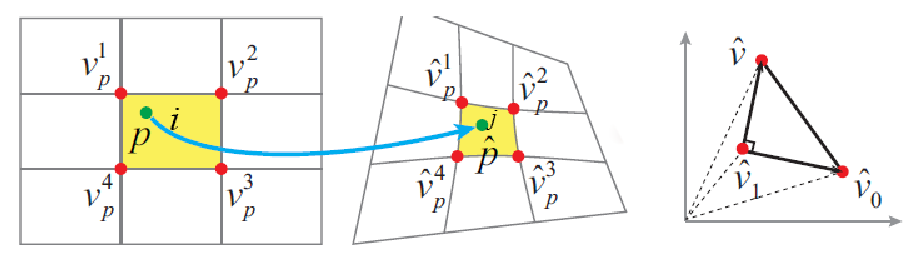
\includegraphics[width=0.75\textwidth]{ch4/asapN.eps}
  \par \quad\quad\quad(a)\quad\quad\quad\quad\quad\quad\quad\quad\quad\quad\quad\quad(b)
% figure caption is below the figure
\end{center}
\caption{(a) The data term is defined according to the fact that a pair of matched features (p, \^{p}) should be represented by the same bilinear interpolation of their four enclosing vertices. (b) The smooth term requires each triangle follow a similarity transformation. The images are borrowed from Ref.~\citenum{Liu_2013ASAP}.}
\label{fig:2}       % Give a unique label
\end{figure}
The corresponding matched feature points \(p\) and $\hat{p}$ in the two frames are within the cells \(i\) and \(j\), respectively. The four corners of cells \(i\) and \(j\) are denoted as ${V}_{p}=[{v}^{1}_{p}$,${v}^{2}_{p}$,${v}^{3}_{p}$,${v}^{4}_{p}]$ and ${\hat{V}_{p}}=[\hat{v}^{1}_{p}$,$\hat{v}^{2}_{p}$,$\hat{v}^{3}_{p}$,$\hat{v}^{4}_{p}]$, respectively. Thus, \(p\) can be expressed as the bilinear interpolation of the four corners of cell \(i\), $p=\sum_{p}{{V}_{p}{w}_{p}}$ .The warping is solved via minimizing the energy function composed of the data term ${E}_{d}$ and smooth term ${E}_{s}$.
${E}_{d}$ is defined as
$${E}_{d}(\hat{V}) = \sum_{p}{\parallel\hat{V}_{p}{w}_{p}- \hat{p}\parallel}^{2} \eqno{(1)},$$
which makes sure the \(p\) and $\hat{p}$ have the same bilinear interpolation of their corresponding cell corners. And ${E}_{s}$ is defined as
$${E}_{s}(\hat{V} )= \sum_{\hat{v}}\parallel\hat{v}-\hat{v}_{1} - s{R}_{90}(\hat{v}_{0} - \hat{v}_{1})\parallel^{2}, s=\frac{\parallel{v}-{v}_{1}\parallel}{\parallel{v}_{0}-{v}_{1}\parallel},{R}_{90} = \left(\begin{array}{cc}{0} &{1} \\{-1} &{0}\end{array}\right),$$
which is a shape-preserving term, that requires the triangle of the neighbour vertices to follow a similarity transformation.  The overall energy combines the data term and smooth term, with a weight factor $\alpha$ to control the amount of regularization.
$$E(\hat{V}) = {E}_d(\hat{V}) + \alpha{E}_{s}(\hat{V}).\eqno{(2)}$$
Since the energy function is a quadric, the warped position of the corner vertices $\hat{Vp}$ can be obtained by solving the sparse linear system. For each cell, a homography is determined by the four corner vertices . The motion of the whole frame is represented by a set of spatially-variant homographies on a 2D grid \cite{Liu_2013ASAP}, which is more robust compared with other methods using only one global homography.\par
 In Eq.(2), the number of the date term constraints will linearly increase with the number of the matched feature points. Large number of the matched feature points may slow down the solving of the sparse linear system. For this reason, we propose to estimate the homographies for cells that contain sufficient feature points. For these cells, denoted as $h$, the date term is defined as,
 $$E^{h}_{d}(\hat{V}) = \sum_{p\in h}{\parallel H_{p}V_{p} - \hat{V_{p}}\parallel}^2$$
where $H_{p}$ is the estimated homography of the cell that encloses $p$. The minimum number of matched feature points to estimate a $3\times3$ homography is 4, in our implementation, we set it as 10 for robust estimation.  For those cells do not meet the minimum matched feature points requirement for homography estimation, we use the bilinear interpolation based data  term as in Eq.(1). Finally, the data term in our warping algorithm is defined as,
$${E}_{d}(\hat{V}) = \sum_{p \notin h}{\parallel\hat{V}_{p}{w}_{p}- \hat{p}\parallel}^{2} +
\sum_{p\in h}{\parallel {H_{p}V_{p} - \hat{V_{p}}}\parallel}^2.$$
To select the proper weight coefficient \(\alpha\) in Eq.(2), the authors in Ref.~\citenum{Liu_2013ASAP} equally discretized $\alpha$ into 10 values between 0.3 and 3. The one with the minimum warping error is selected at last. This method is inefficient. Different to their method, our method adaptively sets the weight coefficient for cells  $c \in h$ using the warping error, $e_{c} = {\parallel H_{c}p_{c} - \hat{p_{c}} \parallel}^2 $, as follows, $\alpha_{c\in h} = s_{1}\exp({e_{c}/avgErr})+ s_{2}$, where $s_{1}$ is set to 0.15, $avgErr$ is the average warping error of $h$, and $s_{2}$ is a truncation factor making $\alpha_{h} \in [0.3,3.0]$. We set $\alpha_{c \notin h}$ to a constant value 1.0. In this way, the data term  is trusted more for the cells with a smaller fitting error, while the stronger regularization is performed on cells with a less reliable homography.
\subsection{Superpixel-based seeded region growing}
\label{sec:3.2}
Considering the heavy computation cost of the dense optical flow, we use KLT-based sparse optical flow with SSRG to get a raw foreground segmentation. Since the pixel-level camera motion has already been estimated in the ASAP warping, we can obtain the superpixel-level camera motion by the average motion of pixels within a superpixel. Then this estimated camera motion is compared with the superpixel-level optical flow. Ideally, the optical flows of background pixels should be identical with the camera motion. If the difference between these two motions is within a threshold, we use a small threshold in practice, e.g., 0.4, these superpixels are labeled as the background seeds. Considering the spatial coherence, we propose the SSRG algorithm, see $Algorithm 1$, to extend these sparse seeds to the entire image frame. The proposed SSRG algorithm is similar to Ref.~\citenum{seededRegionGrowing}, but the main differences are two-fold. (1) The purposes of these two algorithms are different, the algorithm in Ref.~\citenum{seededRegionGrowing} aims to segment the input image into multiple homogenous regions, while our SSRG algorithm divides the image into two regions of the background and the foreground, (2) Our SSRG algorithm is based on superpixels, thus is more efficient than the pixel-based approach in Ref.~\citenum{seededRegionGrowing}.

\renewcommand{\algorithmcfname}{算法}
\begin{algorithm}
\caption{Superpixel-based seeded region growing}
\label{ch4:alg:ssrg}
\LinesNumbered
\KwData {$superpxiels$ of image $I$, background $seeds$, $threshold_{rg}$ for region growing}
\KwResult {background $mask$}
 $\forall p \in superpixels$, $mask[p] \leftarrow 0$ , $segmented[p] \leftarrow 0$ \;
\ForEach {$s$ in $seeds$}{
  $mask[s] \leftarrow 1$ \;
 {$regColor \leftarrow  Color(s)$ \;}
 {$dist \leftarrow 0 ,  regSize \leftarrow 1$ \;}
 {$list \leftarrow empty$ \;}
\While {$dist < threshold_{rg}$ and $regSize < \sharp Superpixels$}{
\ForEach {$p \in $ Neighbors of $s$}{
\If{ $!segmented[p]$ and $p \notin list $}{
 { add $p$ into $list$ \;}
}
}
 $\hat{m} \leftarrow  arg\min_{m \in list}{\parallel regColor - Color(m) \parallel}$ \;
 $  mask[\hat{m}] \leftarrow 1, segmented[\hat{m}] \leftarrow 1$ \;
 $dist \leftarrow \parallel regColor - {Color(\hat{m})} \parallel $ \;
 $regColor = \frac {regColor \times regSize + Color(\hat{m})}  {regSize + 1 }$ \;
 $regSize \leftarrow regSize$ $+ 1$ \;
 remove $\hat{m}$ from $list$
\If {$list$ is empty}{
 $break$\;
}
}
}

\end{algorithm}

An example of $Algorithm 1$ is shown in Figure 3. From left to right, the first two images in Figure 3 are the superpixel segmentations of frames 41 and 42 of the cars4 video in Ref.~\citenum{HopKinsDataSet}. In the third image, the background superpixel seeds are marked in white color. The output of $Algorithm 1$ is shown in the last image.
% For one-column wide figures use
\begin{figure*}[!htbp]
\begin{center}
% Use the relevant command to insert your figure file.
% For example, with the graphicx package use
 % \includegraphics[width=0.22\textwidth]{lsuperpixel.png}\quad
%  \includegraphics[width=0.22\textwidth]{superpixel.png}\quad
%  \includegraphics[width=0.22\textwidth]{seeds.png}\quad
%  \includegraphics[width=0.22\textwidth]{motionCue.png}\\
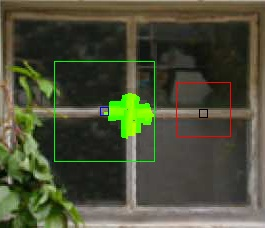
\includegraphics[width=0.9\textwidth]{ch4/fig3.eps}\\
  (a)\quad\quad\quad\quad\quad\quad\quad\quad(b)\quad\quad\quad\quad\quad\quad\quad\quad(c)\quad\quad\quad\quad\quad\quad\quad\quad(d)
% figure caption is below the figure
\end{center}

\caption{An example of the proposed SSRG algorithm. (a) superpixel of $frame_{t-1}$, (b) superpixel of $frame_{t}$, (c) background seeds, (d) result of SSRG.}
\label{fig:3}       % Give a unique label
\end{figure*}
\subsection{Sample consensus appearance model}
\label {sec:3.3}
Our appearance background model is based on multiple samples of color and LBSP feature of each pixel as in Ref.~\citenum{subsenseTIP}. Let $B(x)$ be the background samples of pixel $I(x)$, follow the definition in Ref.~\citenum{subsenseTIP}, the size of $B(x)$ is 50. In the model matching process, the color and LBSP of $I(x)$ are compared with the samples in $B(x)$. If the distance between $I(x)$ and some sample $B(x)[i]$ is within  $T(x)$, $B(x)[i]$ is viewed as a matched sample. If the number of the matched samples exceeds $ T_{n}$, then $I(x)$ will be labeled as the background pixel. $T_{n}$ is set to 2 for all the pixels, and $T(x)$ is a pixel-level threshold controls the maximum difference allowed to match a pixel with a background sample. In Refs.~\citenum{pbas,subsenseTIP}, a feedback mechanism was introduced to dynamically adjust $T(x)$. In Ref.~\citenum{subsenseTIP}, the threshold for the color space and feature space is controlled by an abstract per-pixel variable $R(x)$,
$$T_{color}(x) = R(x) \cdot R^{0}_{color},$$
$$T_{lbsp}(x) = 2^{R(x)} + R^{0}_{lbsp},$$
where $R^{0}_{color}$ and $R^{0}_{lbsp}$ are the minimum color and LBSP distance thresholds, which are set to 30 and 3 respectively \cite{subsenseTIP}. In our algorithm, $R(x)$ is dynamically updated according to the feedback mechanism as,

$$ R(x) = \begin{cases}  R(x)+v & if \quad {R(x)<(1+2D_{min}(x))}^{2} \\  R(x) - \frac{1 }{v } & otherwise \end{cases}$$
where $D_{min}(x)$ is the normalized minimal distances between the samples in $B(x)$ and $I(x)$ . Different from Ref.~\citenum{subsenseTIP}, in which $v$ is also updated according to the blinking pixels in the foreground labelling results, we simply set $v$ to a constant value of 0.1. This is because, in moving camera cases, blinking pixels are hard to track. We also observed that, for moving camera scenarios, the model update policy should be more aggressive. In our algorithm, the background samples are updating guided by the final foreground/background label results. Unlike Ref.~\citenum{subsenseTIP}, where the model update rate is also a dynamic per-pixel  variable, we employ a simpler way. For the background pixels $I_{B}(x)$, we replace the randomly selected $10\%$ of the samples with $I_{B}(x)$ and its neighbors, and for foreground pixels, only one sample may be replaced on a probability of 50\%. \par
Since the sample based model is pixel-independent, it is suitable for parallel implementation. we implement it on GPU via CUDA. For each pixel $I(x)$ , a single thread is launched to compare it with the samples in $B(x)$. In this thread, $R(x)$ and $T(x)$ are also updated. After the final results obtained by the MRF optimization framework described in the following Section, a model updating thread will be launched for each pixel to update the samples.

\subsection{Superpixel-based MRF Optimization}
\label {sec:3.4}
Till now we've got two raw segmentations from the motion cue and the appearance cue. To refine the final results, a temporal coherent supepixel-based MRF optimization framework is proposed. Our method is inspired by the segmentation improvement algorithm  for the stationary camera background subtraction in Ref.~\citenum{MRF}. Let ${F}_{t}$ be the foreground of the input frame  ${I}_{t}$ at $t$  and $S_{t}$ be the superpixel segmentation. Let ${{F}_{t}}^{M}$ be the foreground of the raw segmentation result from the motion, and ${F_{t}}^{A}$ the foreground of the raw segmentation result from the appearance model. Our goal is to get the final result $F_{t}$ from ${{F}_{t}}^{M}$ and ${{F}_{t}}^{A}$. Following the definition of the superpixel probability in Ref.~\citenum{MRF}, the probability of superpixel $s$ belonging to the foreground can be defined as $$
\hat{P_{t}(s)} = \frac{c\sum_{x \in s}{F_{t}}^{A}(x) + (1-c)\sum_{x \in s}{F_{t}}^{M}(x)}{\vert s \vert}\eqno{(3)}$$
where $c$ is the confidence term of the appearance background model, $\vert\cdot\vert$ computes the number of pixels. We add a linear mapping to increase the detection sensitivity, and the final definition of the foreground probability of superpixel $s$ is
$$P_{t}(s) = min(\theta \cdot \hat{P_{t}(s)},1)$$ in practice, $\theta$ is set to $2.0$. Combines the spatial and temporal coherence and the superpixel probability, we define an energy function like \citenum{graphcut04} as follows:
$$ E(F_{t}(S)) = \lambda_{1}\sum_{s \in S_{t}}{U(F_{t}(s))} +$$
 $$\lambda_{2}\sum_{(s_{t}(i),s_{t}(j))\in N}{V(F_{t}(i),F_{t}(j))}$$
 $$ +\lambda_{3}\sum_{s \in S_{t}}{T(F_{t}(s))} .\eqno{(4)}$$

The first term in Eq.(4) is the unary term defined as
$$ U(F_{t}(s)) = -\ln(P_{t}(s))F_{t}(s) - \ln(1-P_{t}(s))(1-F_{t}(s)), $$
and the spatial coherence is maintained via
$$V(F_{t}(i),F_{t}(j)) = \delta( F_{t}(i) - F_{t}(j)) (v_{1} $$
$$+ v_{2}\cdot e^{(-\frac{\parallel \mu_{t}(i) - \mu_{t}(j)\parallel}{2\beta})})\eqno{(5)}$$
in which  $\delta()$ is a Kronecker delta function, $\mu_{t}(s)$ is the average color of superpixel $s$ at time $t$, $\beta$ is estimated for each image as the average color distance among the adjacent superpixels, $v_{1}$ and $v_{2}$ are two predefined constant coefficients set to 0.3 and 40, respectively.
The last term in Eq.(4) is the temporal coherent term. The foreground object in two adjacent frames is temporal coherent, if a superpixel belongs to the foreground in the previous frame, there's a high probability such that the corresponding superpixel in the current frame remains to be foreground. We use the superpixel-level optical flow described in Section 3.2 to establish a link between the superpixels of two consecutive frames. Let $C_{t}(s)$ be the center point of the superpixel $S_{t}(s)$. The corresponding point $C_{t-1}(s)$ in the previous frame can be obtained via the superpixel flow. The temporal neighbor of the $S_{t}(s)$ in the previous frame is defined as
$$
\hat{S_{t-1}}(s) = arg\;min_{i\in S_{t-1}}(\alpha_{s}\parallel (C_{t-1}(s) - C_{t-1}(i))\parallel + $$
$$(1-\alpha_{s})\parallel \mu_{t-1}(i) - \mu_{t}(s)\parallel),$$
where $\alpha_{s} $ controls the importance of the space difference, we set it as a constant value of 0.9. Then the temporal coherent term in Eq.(4) is defined as
$$ T(f_{t}(s)) = v_{3}(1-\delta(F_{t}(s)-F_{t-1}(\hat{S_{t-1}}(s))))\cdot $$
$$e^{-\frac {\parallel \mu_{t}(s) -\mu_{t-1}(\hat{S_{t-1}}(s)) \parallel}{2\beta}}, $$
where $v_{3}$ is a linear mapping factor to make the three components in Eq.(4) comparable. In our implementation $v_{3}$ is set to 40 as $v_{2}$ in Eq.(5).

% For one-column wide figures use
\begin{figure*}[!htbp]
\begin{center}
% Use the relevant command to insert your figure file.
% For example, with the graphicx package use
  %\includegraphics[width=0.18\textwidth]{modelCue.png}
%  \includegraphics[width=0.18\textwidth]{imotionCue.png}
%  \includegraphics[width=0.18\textwidth]{lastMask.png}
%  \includegraphics[width=0.18\textwidth]{currMask.png}
%  \includegraphics[width=0.18\textwidth]{groundtruth.png}
   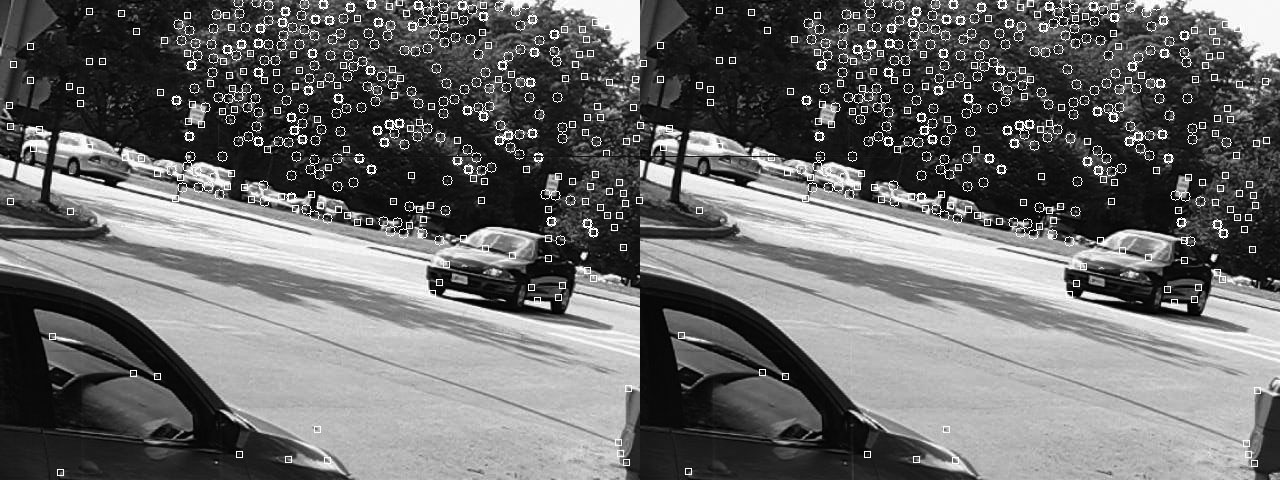
\includegraphics[width=0.9\textwidth]{ch4/fig4.eps}\\
(a)\quad\quad\quad\quad\quad\quad(b)\quad\quad\quad\quad\quad\quad(c)\quad\quad\quad\quad\quad\quad(d)\quad\quad\quad\quad\quad\quad(e)
% figure caption is below the figure
\end{center}

\caption{MRF optimization process, (a) the raw segmentation from the appearance model, (b) the raw segmentation from the motion cue, (c) the foreground labeling result of the last frame, (d) the final result, (e) the ground truth.}
\label{fig:4}       % Give a unique label
\end{figure*}

Finally, the segmentation problem can now be viewed as an energy minimization problem, where we seek $F_{t}(S)$ such that $E(F_{t}(S))$ in Eq.(4) is minimized. This can be done effectively via the graph-cut algorithm \cite{graphcut04}. An example of MRF optimization is shown in Figure 4, where the first two images are the raw segmentation results from the motion cue and the appearance model, the third image is the segmentation result of the last frame, the final result is shown in the last image. \par
Since the energy function is defined in the superpixel level, the computation cost is much lower compared with the pixel-level approach \cite{Multitransform,SubspaceTracking}. The final results of our method is based on the superpixels, all the pixels within a foreground superpixel will be labeled as the foreground, so the size of superpixels in our implementation is relatively small, about 25 pixels on average.

 \section{实验结果与分析}
 \label{ch4:sec:results}
 \subsection{Part A}
We have tested the proposed algorithm on the test video sequences from Hopkins dataset \cite{HopKinsDataSet} (cars1-8, people1-2) and Ref. ~\citenum{ParticleCVPR06} (vcar, vperson) that have been used in \cite{iccv2009,LimPRFloating,Multitransform,kwak2011Generalized} on the same topic. Some of the ground truth images are provided by the datasets \cite{HopKinsDataSet}, the rest ones were manually generated by extracting all the moving objects. \par
In our experiments, an $8\times8$ grid is used to divide the input images into 64 cells for ASAP warping, the $threshold_{rg}$ for SSRG in $Algorithm 1$ is set to the average color difference among the adjacent superpixels in each frame. The weighting parameters in Eq.(4) are set as follows: $\lambda_{1} = 0.5, \lambda_{2} = 0.35, \lambda_{3} = 0.15$. The confidence term $c$ in Eq.(3) is set to $0.75$. We keep the same parameter settings for all the experiments. \par
In Figure 5, some of the results are demonstrated and compared with three other state-of-the-art ones \cite{kwak2011Generalized,Multitransform,5.8s}.
\begin{figure*}[!htbp]
\begin{center}
% Use the relevant command to insert your figure file.
% For example, with the graphicx package use
  %\includegraphics[width=0.15\textwidth]{c2.png}
%  \includegraphics[width=0.15\textwidth]{c3.png}
%  \includegraphics[width=0.15\textwidth]{c4.png}
%  \includegraphics[width=0.15\textwidth]{p1.png}
%  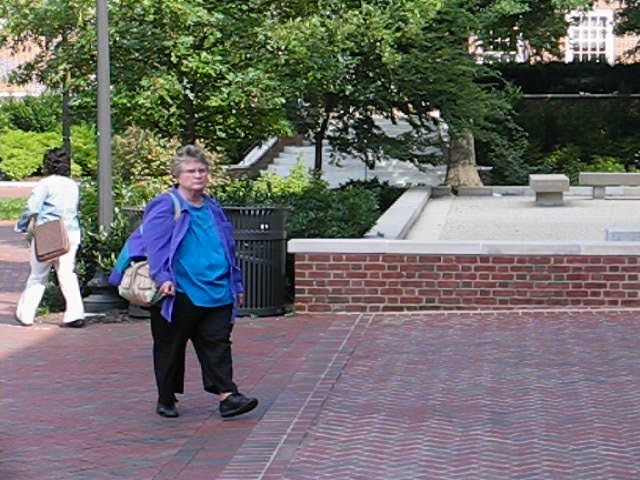
\includegraphics[width=0.15\textwidth]{p2.png}\\
%  \includegraphics[width=0.15\textwidth]{gtc2.png}
%  \includegraphics[width=0.15\textwidth]{gtc3.png}
%  \includegraphics[width=0.15\textwidth]{gtc4.png}
%  \includegraphics[width=0.15\textwidth]{gtp1.png}
%  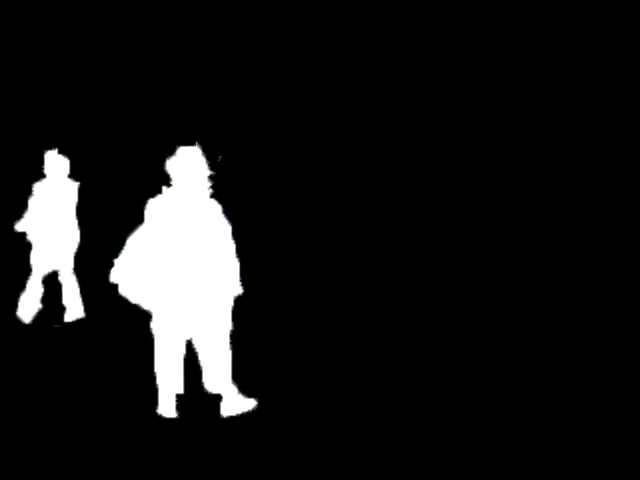
\includegraphics[width=0.15\textwidth]{gtp2.png}\\
%  \includegraphics[width=0.15\textwidth]{c2_m.png}
%  \includegraphics[width=0.15\textwidth]{c3_m.png}
%  \includegraphics[width=0.15\textwidth]{c4_m.png}
%  \includegraphics[width=0.15\textwidth]{p1_m.png}
%  \includegraphics[width=0.15\textwidth]{p2_m.png}\\
%  \includegraphics[width=0.15\textwidth]{c2_k.png}
%  \includegraphics[width=0.15\textwidth]{c3_k.png}
%  \includegraphics[width=0.15\textwidth]{c4_k.png}
%  \includegraphics[width=0.15\textwidth]{p1_k.png}
%  \includegraphics[width=0.15\textwidth]{p2_k.png}\\
%  \includegraphics[width=0.15\textwidth]{c2_mcd.png}
%  \includegraphics[width=0.15\textwidth]{c3_mcd.png}
%  \includegraphics[width=0.15\textwidth]{c4_mcd.png}
%  \includegraphics[width=0.15\textwidth]{p1_mcd.png}
%  \includegraphics[width=0.15\textwidth]{p2_mcd.png}\\
%  \includegraphics[width=0.15\textwidth]{c1_ours.png}
%  \includegraphics[width=0.15\textwidth]{c2_ours.png}
%  \includegraphics[width=0.15\textwidth]{c3_ours.png}
%  \includegraphics[width=0.15\textwidth]{p1_ours.png}
%  \includegraphics[width=0.15\textwidth]{p2_ours.png}\\
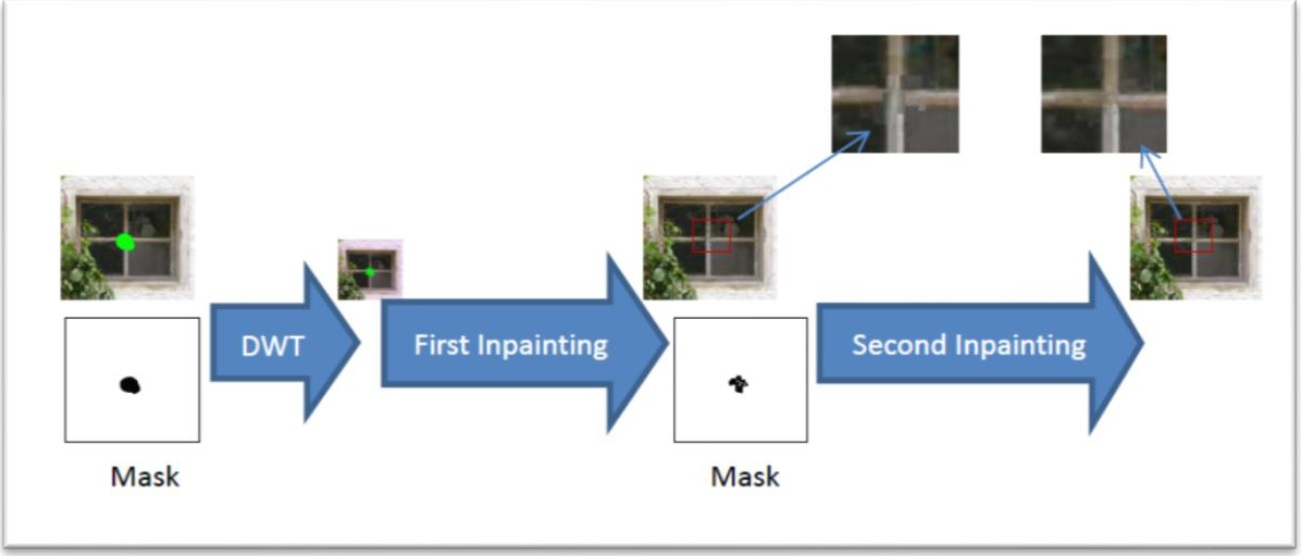
\includegraphics[width=0.9\textwidth]{ch4/fig5.eps}\\

% figure caption is below the figure
\end{center}
\caption{Comparisons with three other algorithms for cars2(20th frame), cars3(19th frame), cars4(40th frame), people1(40th frame) and  people2(16th frame). Row 1 to row 2 show the input frame and the ground truth of moving foreground. Row 3 to row 6 show the results of Refs. ~\citenum{Multitransform,kwak2011Generalized,5.8s}, and ours.}
\label{fig:4}       % Give a unique label
\end{figure*}
The results of Ref.~\citenum{kwak2011Generalized,Multitransform} are copied from Ref.~\citenum{Multitransform}, the implementation of Ref.~\citenum{5.8s} is obtained from the web page of the authors\footnote{https://sites.google.com/site/homekmyi/}. Some of the results are summarized in Table 1. It can be seen that, in most cases, the accuracy of our method outperforms all the three methods in Table 1, and our method achieves the best results on average. The F-score value of our method is slightly higher than Ref.~\citenum{Multitransform}, even though we employ the sparse optical flow and superpixel-level MRF optimization framework.\par
In the first few frames, the results of our method may be noisy. This is because our method relies on the sample-based background model. If the foreground is already in the first frame, it will be initialized into the background model and cause the false foreground results. As our algorithm continues running, these noises will disappear rapidly along with the model updating and the motion-cue-involved global optimization. In the quantitative evaluation of our method, the results of the first 5 frames in each test sequence were ignored. Our motion cue is based on the assumption that the dominant trackable feature points are from the background. For the video frames that violate this assumption, e.g., a close-up view of a walking person, our method would fail.\par


\begin{table*}

% table caption is above the table
\caption{Average $precision(P)$, $recall (R)$, and $F-score (F)$ values for our and state-of-the-art methods. The best scores are denoted in bold. }
\label{tab:1}       % Give a unique label
% For LaTeX tables use
\begin{tabular}{ccccccccccccc} \hline
\multicolumn{1}{c|}{\multirow {2}{*}{}}&\multicolumn{3}{c|}{ours}& \multicolumn{3}{c|}{\citenum{Multitransform}}& \multicolumn{3}{c|}{\citenum{kwak2011Generalized}}& \multicolumn{3}{c}{\citenum{5.8s}}\\
\cline{2-13}
\multicolumn{1}{c|}{}&\multicolumn{1}{c}{P}&\multicolumn{1}{c}{R}&\multicolumn{1}{c|}{F}&\multicolumn{1}{c}{P}&\multicolumn{1}{c}{R}&\multicolumn{1}{c|}{F}&\multicolumn{1}{c}{P}&\multicolumn{1}{c}{R}&\multicolumn{1}{c|}{F}&\multicolumn{1}{c}{P}&\multicolumn{1}{c}{R}&\multicolumn{1}{c}{F}\\
\hline
\multicolumn{1}{c|}{vcar}&\multicolumn{1}{c}{\textbf{0.940}}&\multicolumn{1}{c}{\textbf{0.887}}&\multicolumn{1}{c|}{\textbf{0.913}}&\multicolumn{1}{c}{0.839}&\multicolumn{1}{c}{0.856}&\multicolumn{1}{c|}{0.846}&\multicolumn{1}{c}{0.595}&\multicolumn{1}{c}{0.626}&\multicolumn{1}{c|}{0.607}&\multicolumn{1}{c}{0.690}&\multicolumn{1}{c}{0.365}&\multicolumn{1}{c}{0.478}\\
\multicolumn{1}{c|}{vperson}&\multicolumn{1}{c}{0.757}&\multicolumn{1}{c}{0.898}&\multicolumn{1}{c|}{0.821}&\multicolumn{1}{c}{\textbf{0.823}}&\multicolumn{1}{c}{\textbf{0.936}}&\multicolumn{1}{c|}{\textbf{0.873}}&\multicolumn{1}{c}{0.539}&\multicolumn{1}{c}{0.628}&\multicolumn{1}{c|}{0.568}&\multicolumn{1}{c}{0.753}&\multicolumn{1}{c}{0.476}&\multicolumn{1}{c}{0.583}\\
\multicolumn{1}{c|}{cars1}&\multicolumn{1}{c}{0.757}&\multicolumn{1}{c}{\textbf{0.974}}&\multicolumn{1}{c|}{\textbf{0.852}}&\multicolumn{1}{c}{0.729}&\multicolumn{1}{c}{0.945}&\multicolumn{1}{c|}{0.822}&\multicolumn{1}{c}{\textbf{0.843}}&\multicolumn{1}{c}{0.738}&\multicolumn{1}{c|}{0.785}&\multicolumn{1}{c}{0.527}&\multicolumn{1}{c}{0.379}&\multicolumn{1}{c}{0.441}\\
\multicolumn{1}{c|}{cars2}&\multicolumn{1}{c}{\textbf{0.886}}&\multicolumn{1}{c}{\textbf{0.934}}&\multicolumn{1}{c|}{\textbf{0.910}}&\multicolumn{1}{c}{0.698}&\multicolumn{1}{c}{0.908}&\multicolumn{1}{c|}{0.789}&\multicolumn{1}{c}{0.679}&\multicolumn{1}{c}{0.741}&\multicolumn{1}{c|}{0.705}&\multicolumn{1}{c}{0.282}&\multicolumn{1}{c}{0.131}&\multicolumn{1}{c}{0.179}\\
\multicolumn{1}{c|}{cars3}&\multicolumn{1}{c}{\textbf{0.841}}&\multicolumn{1}{c}{\textbf{0.969}}&\multicolumn{1}{c|}{\textbf{0.901}}&\multicolumn{1}{c}{0.820}&\multicolumn{1}{c}{0.956}&\multicolumn{1}{c|}{0.882}&\multicolumn{1}{c}{0.804}&\multicolumn{1}{c}{0.802}&\multicolumn{1}{c|}{0.802}&\multicolumn{1}{c}{0.505}&\multicolumn{1}{c}{0.236}&\multicolumn{1}{c}{0.322}\\
\multicolumn{1}{c|}{cars4}&\multicolumn{1}{c}{\textbf{0.951}}&\multicolumn{1}{c}{\textbf{0.932}}&\multicolumn{1}{c|}{\textbf{0.942}}&\multicolumn{1}{c}{0.877}&\multicolumn{1}{c}{0.917}&\multicolumn{1}{c|}{0.895}&\multicolumn{1}{c}{0.575}&\multicolumn{1}{c}{0.679}&\multicolumn{1}{c|}{0.621}&\multicolumn{1}{c}{0.502}&\multicolumn{1}{c}{0.251}&\multicolumn{1}{c}{0.335}\\
\multicolumn{1}{c|}{cars5}&\multicolumn{1}{c}{\textbf{0.926}}&\multicolumn{1}{c}{0.777}&\multicolumn{1}{c|}{0.845}&\multicolumn{1}{c}{0.892}&\multicolumn{1}{c}{\textbf{0.857}}&\multicolumn{1}{c|}{\textbf{0.874}}&\multicolumn{1}{c}{0.623}&\multicolumn{1}{c}{0.680}&\multicolumn{1}{c|}{0.645}&\multicolumn{1}{c}{0.659}&\multicolumn{1}{c}{0.138}&\multicolumn{1}{c}{0.228}\\
\multicolumn{1}{c|}{cars6}&\multicolumn{1}{c}{0.866}&\multicolumn{1}{c}{\textbf{0.988}}&\multicolumn{1}{c|}{\textbf{0.923}}&\multicolumn{1}{c}{\textbf{0.868}}&\multicolumn{1}{c}{0.942}&\multicolumn{1}{c|}{0.903}&\multicolumn{1}{c}{0.624}&\multicolumn{1}{c}{0.890}&\multicolumn{1}{c|}{0.731}&\multicolumn{1}{c}{0.584}&\multicolumn{1}{c}{0.140}&\multicolumn{1}{c}{0.226}\\
\multicolumn{1}{c|}{cars7}&\multicolumn{1}{c}{0.714}&\multicolumn{1}{c}{\textbf{0.974}}&\multicolumn{1}{c|}{0.824}&\multicolumn{1}{c}{\textbf{0.802}}&\multicolumn{1}{c}{0.950}&\multicolumn{1}{c|}{\textbf{0.869}}&\multicolumn{1}{c}{0.662}&\multicolumn{1}{c}{0.729}&\multicolumn{1}{c|}{0.691}&\multicolumn{1}{c}{0.282}&\multicolumn{1}{c}{0.311}&\multicolumn{1}{c}{0.296}\\
\multicolumn{1}{c|}{cars8}&\multicolumn{1}{c}{\textbf{0.793}}&\multicolumn{1}{c}{\textbf{0.945}}&\multicolumn{1}{c|}{\textbf{0.862}}&\multicolumn{1}{c}{0.737}&\multicolumn{1}{c}{0.944}&\multicolumn{1}{c|}{0.826}&\multicolumn{1}{c}{0.775}&\multicolumn{1}{c}{0.766}&\multicolumn{1}{c|}{0.767}&\multicolumn{1}{c}{0.529}&\multicolumn{1}{c}{0.699}&\multicolumn{1}{c}{0.602}\\
\multicolumn{1}{c|}{people1}&\multicolumn{1}{c}{\textbf{0.947}}&\multicolumn{1}{c}{\textbf{0.879}}&\multicolumn{1}{c|}{\textbf{0.912}}&\multicolumn{1}{c}{0.925}&\multicolumn{1}{c}{0.816}&\multicolumn{1}{c|}{0.866}&\multicolumn{1}{c}{0.492}&\multicolumn{1}{c}{0.693}&\multicolumn{1}{c|}{0.563}&\multicolumn{1}{c}{0.760}&\multicolumn{1}{c}{0.393}&\multicolumn{1}{c}{0.518}\\
\multicolumn{1}{c|}{people2}&\multicolumn{1}{c}{\textbf{0.950}}&\multicolumn{1}{c}{\textbf{0.981}}&\multicolumn{1}{c|}{\textbf{0.965}}&\multicolumn{1}{c}{0.939}&\multicolumn{1}{c}{0.895}&\multicolumn{1}{c|}{0.916}&\multicolumn{1}{c}{0.850}&\multicolumn{1}{c}{0.774}&\multicolumn{1}{c|}{0.808}&\multicolumn{1}{c}{0.728}&\multicolumn{1}{c}{0.425}&\multicolumn{1}{c}{0.537}\\
\hline
\multicolumn{1}{c|}{average}&\multicolumn{1}{c}{\textbf{0.860}}&\multicolumn{1}{c}{\textbf{0.928}}&\multicolumn{1}{c|}{\textbf{0.889}}&\multicolumn{1}{c}{0.829}&\multicolumn{1}{c}{0.910}&\multicolumn{1}{c|}{0.868}&\multicolumn{1}{c}{0.670}&\multicolumn{1}{c}{0.729}&\multicolumn{1}{c|}{0.698}&\multicolumn{1}{c}{0.597}&\multicolumn{1}{c}{0.333}&\multicolumn{1}{c}{0.428}\\
\hline

\end{tabular}
\end{table*}


\begin{table}
\caption{Comparisons of computation speed and foreground detection accuracy}
\label{tab:2}       % Give a unique label
\begin{tabular}{cccc}

  \hline
  % after \\: \hline or \cline{col1-col2} \cline{col3-col4} ...
  Algorithm & Preprocessing & Speed & F-score \\
\hline
  \citenum{Multitransform} & Dense Optical Flow & NA & 0.848 \\
  \citenum{gbsuperpixel} & Dense Optical Flow & 0.17fps & 0.923 \\
  \citenum{5.8s} & No  & 45fps & 0.419 \\
  ours & No & 7.65fps & 0.910 \\
  \hline

\end{tabular}
\begin{tabular}{c}
\end{tabular}
\end{table}

%\begin{table}
%\caption{Comparison of computation time}
%\label{tab:2}
%\begin{tabular}
%  \hline
%  % after \\: \hline or \cline{col1-col2} \cline{col3-col4} ...
%  Algorithm & Preprocessing & Speed & Accuracy \\
%  \cite{GbsSuperpixel} & Dense Optical Flow & 0.17fps & ? \\
%  \cite{SubspaceTracking} & Dense Point Trajectories & 0.55fps & ? \\
%  \cite{5.8s} & No  & 170fps & ? \\
%  ours & No & 20fps @320*240 & ? \\
%  \hline
%\end{tabular}
%\end{table}
% For one-column wide figures use
\begin{figure}[!htbp]
\begin{center}
% Use the relevant command to insert your figure file.
% For example, with the graphicx package use
  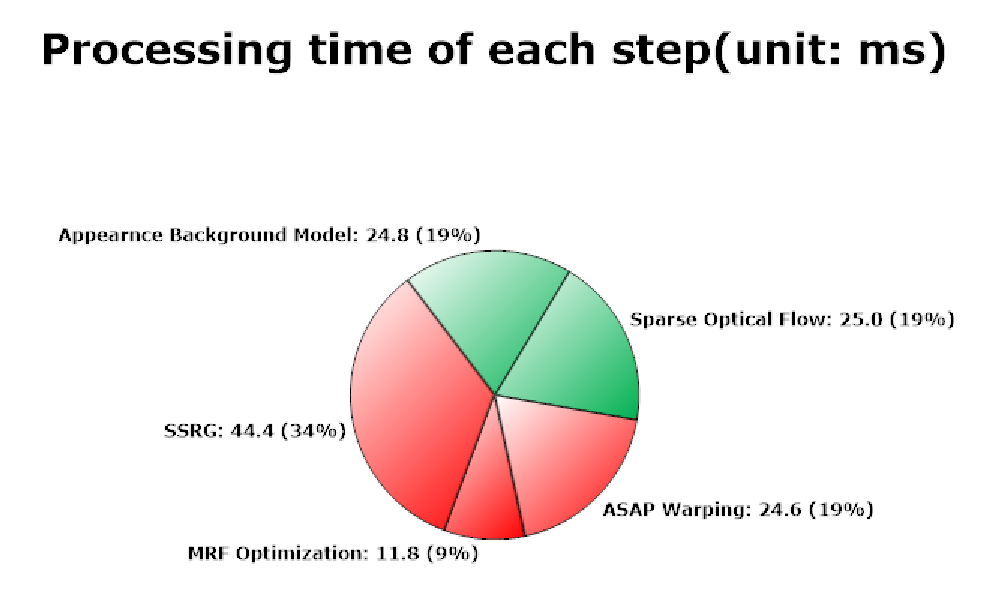
\includegraphics[width=0.8\textwidth]{ch4/fig6.eps}

% figure caption is below the figure
\end{center}

\caption{The processing time of each step of the proposed algorithm for $640\times480$ size input, steps implemented on GPU are denoted in green, others are in red.}
\label{fig:5}       % Give a unique label
\end{figure}
As for the computation speed, our algorithm runs at about 8 FPS with the frame size 640$\times$480 input on a PC with an Intel i7 CPU and a Nvidia Geforce Titan GPU. The processing time for each step of the proposed algorithm is shown in Figrue 6. The GPU implementation of KLT algorithm in OpenCV is adopted to calculate the sparse optical flows, and our appearance background model is also implemented on GPU. As SSRG and MRF optimizations are implemented on the superpixel level,  these two operations are quite fast. Based on the sparse optical flow and SSRG, our method only takes about $70ms$ to obtain a raw segmentation of foreground from the motion cue. The comparisons of the computation speeds between our method and the other state-of-the-art methods with dense optical flow are summarized in Table 2. The speeds and F-score values of the other methods are imported from their papers. For a fair comparison, in Table 2, the F-score value of each method is the average F-score of the four test sequences from \cite{HopKinsDataSet}(cars1, cars2, people1, people2) that were used in Refs.~\citenum{Multitransform,gbsuperpixel}. The original frame size of all the four test sequences is $640\times480$. The computation speed in Ref.~\citenum{Multitransform} could not be found in their paper. Compared with Ref.~\citenum{gbsuperpixel}, our method is about 45 times faster in speed with a sightly lower F-score. The method proposed in Ref.~\citenum{5.8s} is a very fast algorithm running in real time even on a smart-phone platform, but the accuracy is much lower than other methods in Table 2, and this limits its usage in applications that require high accuracy. A significant advantage of our method is that it can be used in a plug-and-play way for many near-real-time applications.
\subsection{Part B}
In this part, we validate the proposed algorithm on the CD.Net 2014 Dataset\cite{CD2014}. Firstly, our algorithm is tested on the PTZ(Pan-Tile-Zoom) category. In this category, there are four long videos captured by PTZ cameras. The average length of the four sequences is 2158 frames. We use the same parameter settings as described in Part A. For the objective evaluation, we use the same performance metrics in Ref.~\citenum{CD2014}. In addition, PSNR(Peak Signal Noise Ratio) and NCC(Normalized Cross-Correlation) are computed between the segmentation result and the ground truth as follows $$MSE=\frac{1}{M\times N}\sum_{x,y}\left \| I_{x,y}-J_{x,y} \right \|^{2},PSNR = 20\times log_{10}\left ( \frac{255}{\sqrt{MSE}}\right )$$
$$NCC=\frac{\sum_{x,y}\left( I_{x,y}-\bar J_{x,y}\right )\left(J_{x,y}- \bar I_{x,y} \right )}{M\times N\times Std(I) \times Std(J)}$$ where $M$ and $N$ are the image width and height, $\bar I_{x,y},\bar J_{x,y}$ are the mean value of image $I$ and $J$ respectively, $Std$ stands for the standard deviation operation.\par
 In Table 3, the quantity evaluation results are listed and compared with other state-of-the-art algorithms. Our algorithm, named as FMCBS,  ranks the top on the PTZ category of the CD.Net 2014 Dataset\cite{CD2014} when submitting this paper \footnote{http://wordpress-jodoin.dmi.usherb.ca/results2014/412/}. The ranking is computed by the average ranking on the 7 metrics. The definition of these metrics, Recall(R), Sp(Specificity), FPR(False Positive Rate), FNR(False Negative Rate), PWC(Percentage of Wrong Classification), F(F-score) and P(Precision) can be found in Ref.~\citenum{CD2014}.

 \begin{table}[ht]
\caption{Comparisons with other state-of-the-art algorithms on the PTZ category of the CD.Net 2014 DataSet\cite{CD2014}.}
\label{tab:Comparisons on PTZ }
\begin{center}
\begin{tabular}{|l|l|l|l|l|l|l|l|l|l|l|} %% this creates two columns
%% |l|l| to left justify each column entry
%% |c|c| to center each column entry
%% use of \rule[]{}{} below opens up each row
\hline
\rule[-1ex]{0pt}{3.5ex}  Method & Ranking & R &Sp & FPR & FNR &PWC &F &P & NCC & PSNR \\
\hline
\rule[-1ex]{0pt}{3.5ex}  FMCBS & 3.86 & 0.834 & 0.998 & 0.003 & 0.167 &0.384&0.704&0.645 &0.194&27.654\\
\hline
\rule[-1ex]{0pt}{3.5ex}  PAWCS\cite{Stcharles2015A}&9.43&0.698&0.991&0.009&0.302&1.116&0.461&0.473&0.155&17.657 \\
\hline
\rule[-1ex]{0pt}{3.5ex}  SharedModel\cite{Chen2015Learning}&  11.71&0.797&0.979&0.021&0.203&2.217&0.386&0.312&0.174&12.392  \\
\hline
\rule[-1ex]{0pt}{3.5ex}  SuBSENSE\cite{subsenseTIP}&  13.43&0.831&0.963&0.037&0.169&3.816&0.348&0.284&0.193&15.992 \\
\hline
\rule[-1ex]{0pt}{3.5ex}  CwisarDH\cite{Gregorio2014Change}&13.57&0.336&0.998&0.002&0.664&0.685&0.322&0.482&0.105&18.708  \\
\hline
\end{tabular}
\end{center}
\end{table}


To show the extensibility of the proposed algorithm. We have also tested our algorithm on two challenging sequences, boats and canoe, from the dynamic background category in the CD.Net 2014 dataset. These two video sequences are captured by a static camera with dynamic background contents. For these sequences, the same model updating policy is used as Ref.~\citenum{subsenseTIP}. Since the camera is static, only the appearance cue is used. In Table 4, the performance of the proposed algorithm is compared with other state-of-the-art sample-based background model algorithms. Only using a single background image, the algorithm proposed in Ref.~\cite{Chien2002Efficient} can not effectively handle the dynamic background in the videos, and it has the worst performance compared with other algorithms in Tabel 4. It is shown that our algorithm outperforms the original SuBSENSE algorithm \cite{subsenseTIP} in terms of F-score, this contributes to our MRF optimization framework.

 \begin{table}[ht]
\caption{Comparisons with other related algorithms on boats and canoe video in dynamic background category of the CD.Net 2014 Dataset \cite{CD2014}.}
\label{tab:Comparisons on Dynamic backgrounds }
\begin{center}
\begin{tabular}{|l|l|l|l|l|l|l|l|l|l|l|} %% this creates two columns
%% |l|l| to left justify each column entry
%% |c|c| to center each column entry
%% use of \rule[]{}{} below opens up each row
\hline
\rule[-1ex]{0pt}{3.5ex}  Method &R &Sp & FPR & FNR &PWC &F &P\\
\hline
\rule[-1ex]{0pt}{3.5ex}  EMOS\cite{Chien2002Efficient}&  0.240&0.987&0.013&0.760&1.993&0.184&0.150 \\
\hline
\rule[-1ex]{0pt}{3.5ex}  PBAS\cite{pbas}&0.359&1.000&0.000&0.641&0.604&0.527&0.992  \\
\hline
\rule[-1ex]{0pt}{3.5ex}  SuBSENSE\cite{subsenseTIP}&  0.600&1.000&0.000&0.400&0.408&0.734&0.945 \\
\hline
\rule[-1ex]{0pt}{3.5ex}  FMCBS &  0.734 & 0.999 & 0.001 & 0.257 &0.319&0.814&0.899\\
\hline
\rule[-1ex]{0pt}{3.5ex}  PAWCS\cite{Stcharles2015A}&0.844&0.999&0.001&0.156&0.211&0.882&0.924\\
\hline
\end{tabular}
\end{center}
\end{table}
 \section{本章小结}
 \label{ch4:sec:conclusions}
 In this paper, a fast background subtraction algorithm for freely moving cameras is proposed. Our method mainly relies on two kinds of cues to effectively detect foreground objects in videos captured by moving cameras. The first cue is based on the sample consensus appearance model, in which ASAP warping technique is adopted to robustly estimate and compensate the camera motions. Then the warped frame is compared with the background model to get the raw segmentations for the image frames. On the other hand, another important cue to distinguish the foreground is that the motion of the foreground is different from the motion induced by the camera. Comparing these superpixel flows with the estimated camera motion, some sparse background seeds can be obtained. Another raw segmentation can be obtained by extending these seeds to the entire frame via the proposed SSRG algorithm.  To refine these raw results, a superpixel-based  temporal coherent MRF optimization framework is built, and the final foreground/background labelling is obtained via the graph-cut algorithm. Our method does not rely on any preprocessing steps for computing the dense optical flows or point trajectories, it is simple and easy to implement. Extensive experiments show that the proposed algorithm achieves the state-of-the-art foreground detection accuracy, while being much faster than other competing methods.
